\chapter{Introduction}
\label{ch:Introduction}

\section{General}


\section{Goals}


\section{Motivation}


\section{GaitWatch}

This paragraph will describe the hardware we used..

The GaitWatch device \cite{olivares_vicente_gaitwatch_2013} is a MIMU designed to monitor the motion of patients while attached to the body. It was developed at the Department of Neurology of the Ludwig-Maximilians University in Munich in conjunction with the Department of Signal Theory, Telematics and Communications of the University of Granada. The system is composed of a set of embedded magnetic and inertial sensors wired to a box containing a microcontroller. This microcontroller is in charge of collecting data from the embedded box sensors, as well as from the external measurement units, and storing them on a memory card. The various units are placed at the patient's thighs, shanks, arms and trunk as shown in Figure \ref{fig:GaitWatch_placement}. The components of the three different kinds of subunits are described below:


\begin{itemize}

\item \textsc{Type A} -- thighs and shanks: 

IMU Analog Combo Board with 5 Degrees of Freedom \cite{IMU5} containing an IDG500 biaxial gyroscope (from which only Y axis is actually used) with a measurement range of ±500°/s \cite{IDG500} and a ±3g triaxial accelerometer, ADXL335 \cite{ADXL335}.

\item \textsc{Type B} -- arms:

IDG500 biaxial gyroscope with a measurement range of ±500°/s \cite{IDG500}.

\item \textsc{Type C} -- trunk:

ADXL345 triaxial accelerometer with programmable range \linebreak (±2g/±4g/±8g/±16g) \cite{ADXL345},
IMU3000 triaxial gyroscope with programmable range (±250/±500/±1000/±3000°/s) \cite{IMU3000}, 
Micromag3 \allowbreak triaxial magnetometer with a measurement range of ±11Gauss \cite{MicroMag3}, AL-XAVRB board containing an AVR ATxmega processor \cite{AVRATxmega}.

\end{itemize}

\begin{figure}
	\centering
	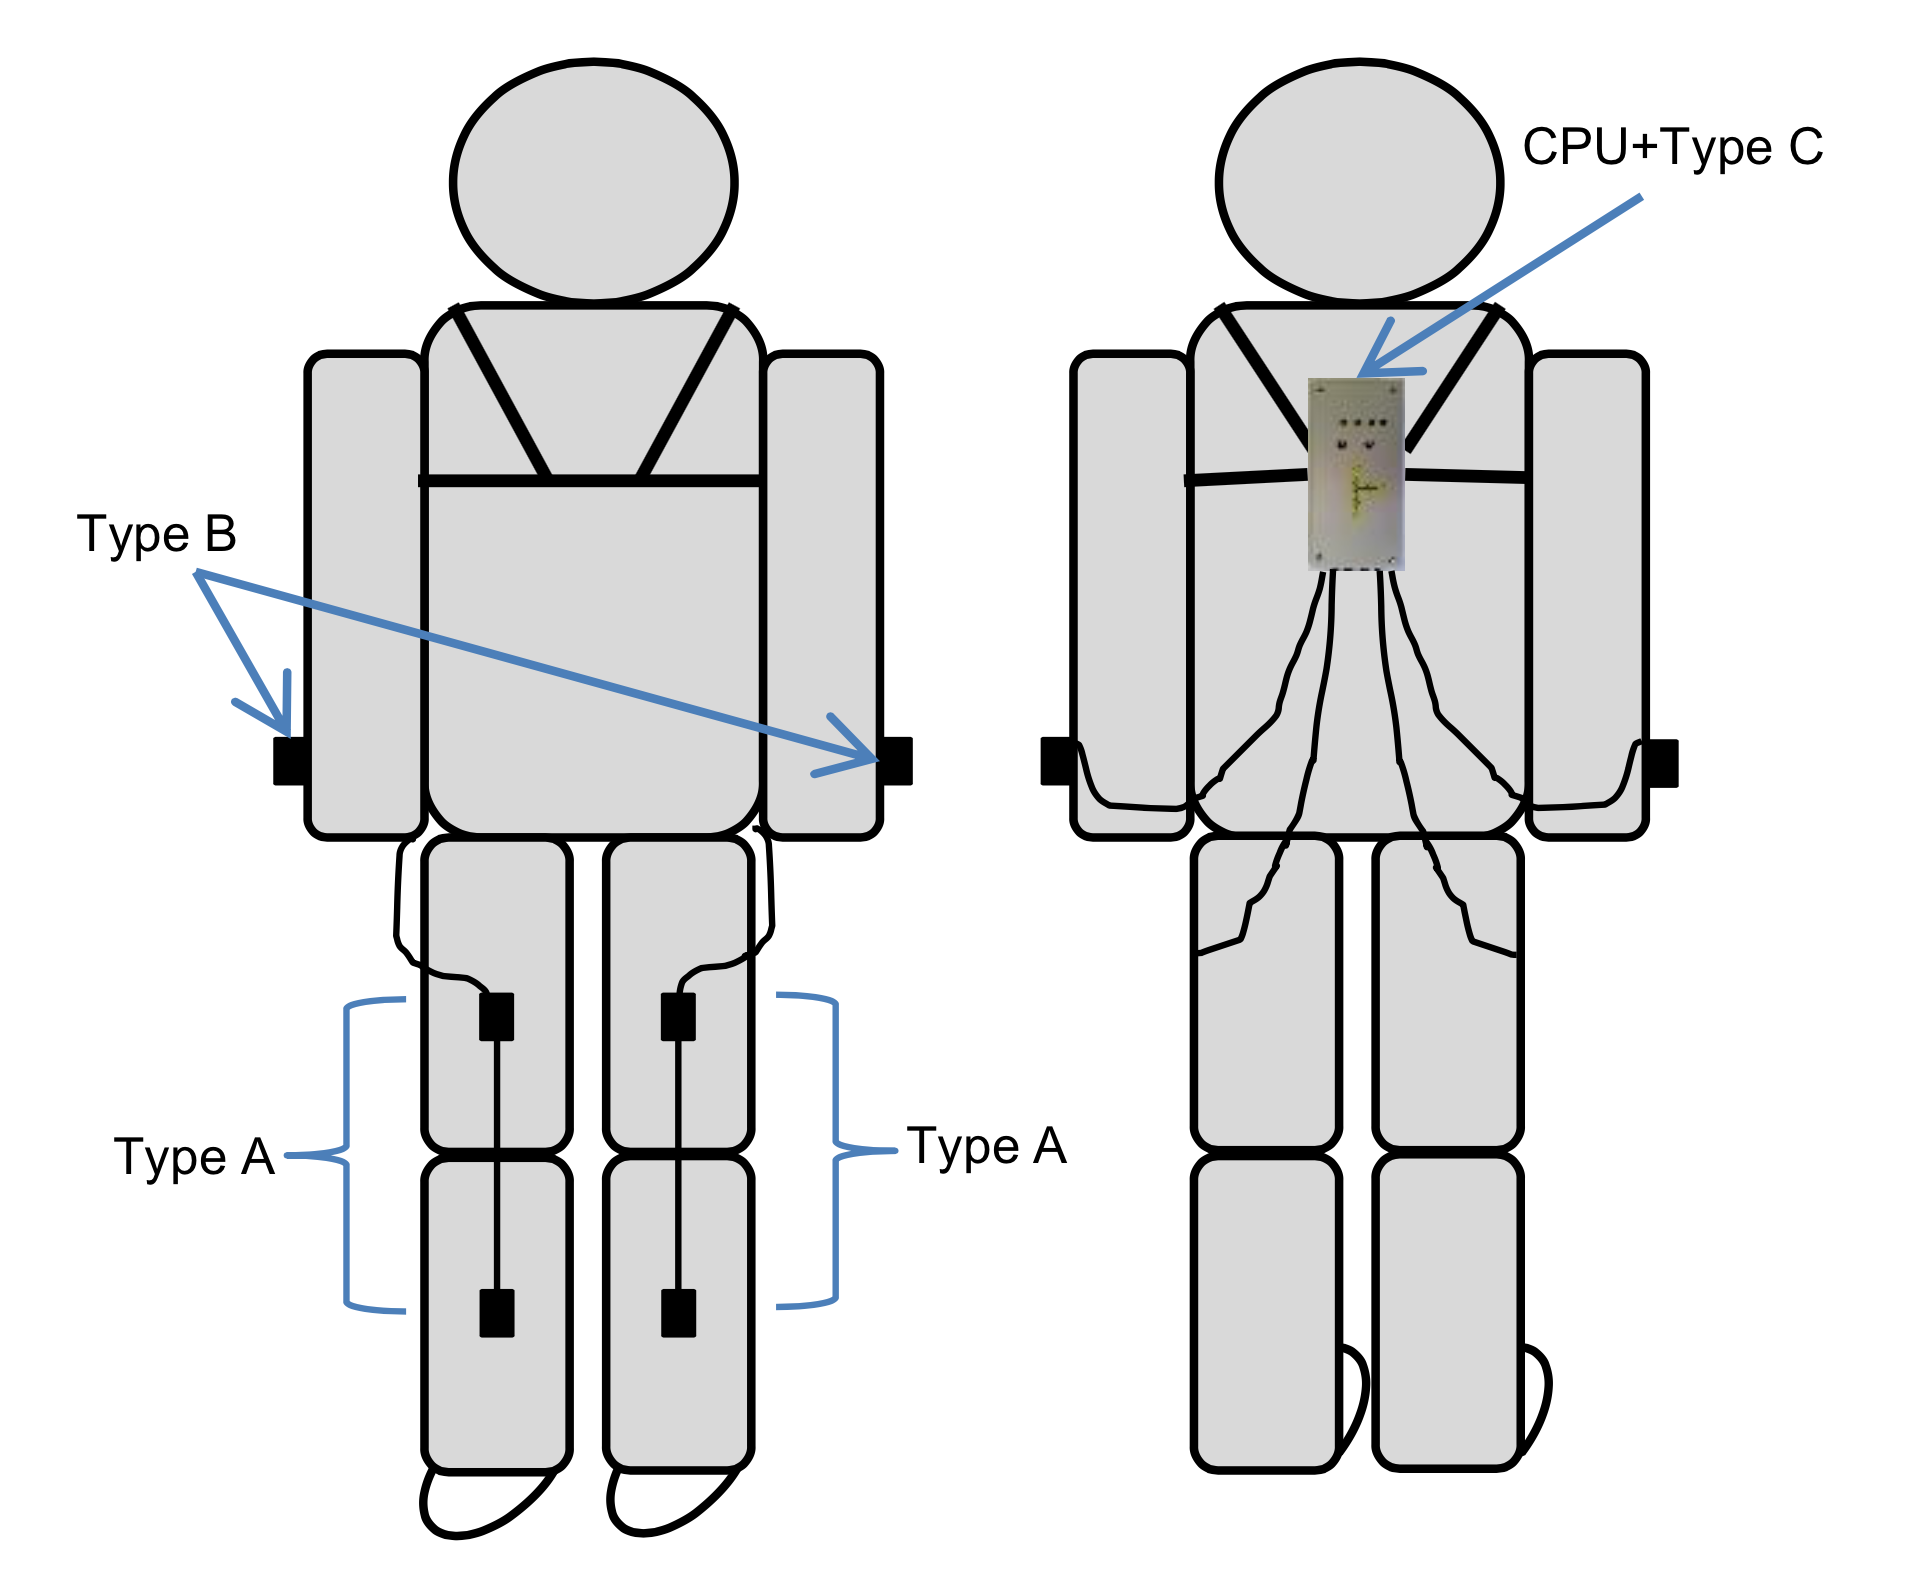
\epsfig{file=images/GaitWatch_placement, width=9cm}
	\caption{Placement of GaitWatch components at the body \cite{olivares_vicente_gaitwatch_2013}.}
	\label{fig:GaitWatch_placement}
\end{figure}

\section{Methodology}

The team in which I was integrated worked using the agile software development methodology. Working software was delivered frequently and was the principal measure of progression. Our self-organising team consisted of three members meeting regularly. Parts of the software were developed doing pair programming. To follow the progress of other team members at any time we used Pivotal Tracker, a tool for agile project management and GitHub, a repository hosting service based on the distributed version control system Git. I used the document markup language \LaTeX{} to write this report.

\section{Document Structure}

Next, in Chapter 2, we will elaborate on the hardware we used and describe the synchronisation process in detail.
